\documentclass[12pt, a4paper, oneside]{article}\usepackage[]{graphicx}\usepackage[]{color}
%% maxwidth is the original width if it is less than linewidth
%% otherwise use linewidth (to make sure the graphics do not exceed the margin)
\makeatletter
\def\maxwidth{ %
  \ifdim\Gin@nat@width>\linewidth
    \linewidth
  \else
    \Gin@nat@width
  \fi
}
\makeatother

\definecolor{fgcolor}{rgb}{0.345, 0.345, 0.345}
\newcommand{\hlnum}[1]{\textcolor[rgb]{0.686,0.059,0.569}{#1}}%
\newcommand{\hlstr}[1]{\textcolor[rgb]{0.192,0.494,0.8}{#1}}%
\newcommand{\hlcom}[1]{\textcolor[rgb]{0.678,0.584,0.686}{\textit{#1}}}%
\newcommand{\hlopt}[1]{\textcolor[rgb]{0,0,0}{#1}}%
\newcommand{\hlstd}[1]{\textcolor[rgb]{0.345,0.345,0.345}{#1}}%
\newcommand{\hlkwa}[1]{\textcolor[rgb]{0.161,0.373,0.58}{\textbf{#1}}}%
\newcommand{\hlkwb}[1]{\textcolor[rgb]{0.69,0.353,0.396}{#1}}%
\newcommand{\hlkwc}[1]{\textcolor[rgb]{0.333,0.667,0.333}{#1}}%
\newcommand{\hlkwd}[1]{\textcolor[rgb]{0.737,0.353,0.396}{\textbf{#1}}}%

\usepackage{framed}
\makeatletter
\newenvironment{kframe}{%
 \def\at@end@of@kframe{}%
 \ifinner\ifhmode%
  \def\at@end@of@kframe{\end{minipage}}%
  \begin{minipage}{\columnwidth}%
 \fi\fi%
 \def\FrameCommand##1{\hskip\@totalleftmargin \hskip-\fboxsep
 \colorbox{shadecolor}{##1}\hskip-\fboxsep
     % There is no \\@totalrightmargin, so:
     \hskip-\linewidth \hskip-\@totalleftmargin \hskip\columnwidth}%
 \MakeFramed {\advance\hsize-\width
   \@totalleftmargin\z@ \linewidth\hsize
   \@setminipage}}%
 {\par\unskip\endMakeFramed%
 \at@end@of@kframe}
\makeatother

\definecolor{shadecolor}{rgb}{.97, .97, .97}
\definecolor{messagecolor}{rgb}{0, 0, 0}
\definecolor{warningcolor}{rgb}{1, 0, 1}
\definecolor{errorcolor}{rgb}{1, 0, 0}
\newenvironment{knitrout}{}{} % an empty environment to be redefined in TeX

\usepackage{alltt} % Paper size, default font size and one-sided paper
%\graphicspath{{./Figures/}} % Specifies the directory where pictures are stored
%\usepackage[dcucite]{harvard}
\usepackage{rotating}
\usepackage{setspace}
\usepackage{pdflscape}
\usepackage[flushleft]{threeparttable}
\usepackage{multirow}
\usepackage[comma, sort&compress]{natbib}% Use the natbib reference package - read up on this to edit the reference style; if you want text (e.g. Smith et al., 2012) for the in-text references (instead of numbers), remove 'numbers' 
\usepackage{graphicx}
%\bibliographystyle{plainnat}
\bibliographystyle{agsm}
\usepackage[colorlinks = true, citecolor = blue, linkcolor = blue]{hyperref}
%\hypersetup{urlcolor=blue, colorlinks=true} % Colors hyperlinks in blue - change to black if annoying
%\renewcommand[\harvardurl]{URL: \url}
\IfFileExists{upquote.sty}{\usepackage{upquote}}{}
\begin{document}
\title{Questions on Calculus}
\author{Rob Hayward} 
\date{\today}
\maketitle

\doublespacing
\begin{enumerate}
\item This is the total physical product curve from last week.  How would you calculate the \emph{average physical product}? 

This would be any line between the origin and the TPP curve, and it is $\frac{TPP}{Q}$.  

\begin{knitrout}
\definecolor{shadecolor}{rgb}{0.969, 0.969, 0.969}\color{fgcolor}

{\centering 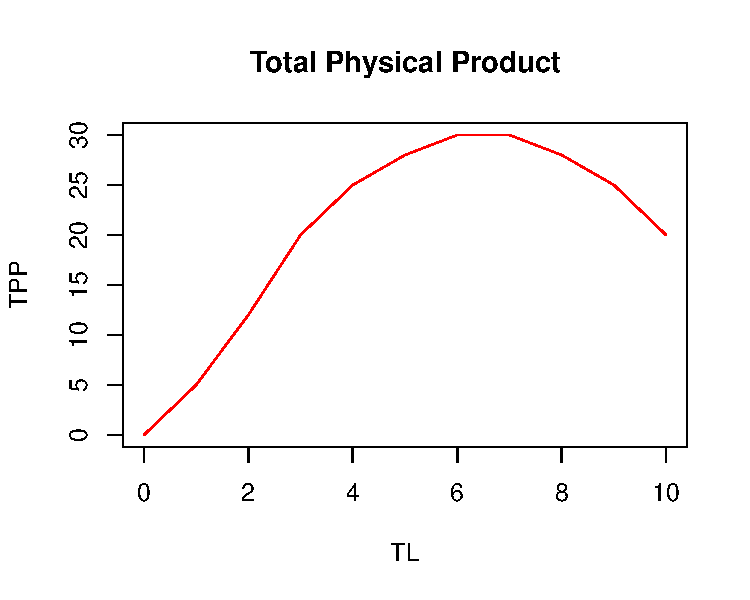
\includegraphics[width=\maxwidth]{figure/plot} 

}



\end{knitrout}

\item How would you calculate the \emph{marginal physical product}?

This is the gradient of the TPP, which would be $\frac{\Delta TPP}{\Delta Q}$

\item What are the drivatives of
\begin{itemize}
\item $y = 2 + 6x$

$y' = 6$

\item $y = 5 - 4x +2x^3$

$y' = -4 + 6x^2$

\item $y = 25 +6x^2 - 3x^3 +25x^4$

$y' =  12x -9x^2 +100x^3$

\item $y - 3 = 2x$

$y' = 2$

\item $TPP = 24 +5Q +2Q^2 - Q^3$

$TPP' =  5 +4Q - 3Q^2$

\item What does your answer to the prevous question tell you about the shape of the Total Physical Product Curve? 

It goes up initially but starts rise at a slower pace.  There are diminishing returns.  

Differentiate

\item $TPP = 15 +15Q +Q^2 - Q^3$

$TPP' = 15 + 2Q - 3Q^2$

\item $TU = 25 + X_1 - X_1^2$

$TU' = 1 - 2X_1$

\item $TU = 25 +25X_1 -2X_1^2$

$TU' = 25 - 4X_1$

\item What does your answer to the previous question tell you about the shape of the Total Utility Curve? 

It shows that the utiity function is concave.  There are diminishing returns. 

\end{itemize}

\item What is the gradient of the TPP at its peak? 

Zero

\item What is the value of the MPP when TPP is at its peak? 

Zero

\item Given the $TPP = 100 + 32Q +10Q^2 - Q^3$, 
\begin{itemize}
\item What is the TPP' or MPP?

$MPP = 32 +20Q - 3Q^2$

\item How would you find the maximum TPP?

Find the value of Q for which the derivative or the MPP is zero. 
\end{itemize}

\item Given the $TPP = 500 + 180Q + 30Q^2 - 2Q^3$, 
\begin{itemize}
\item What is the TPP' or MPP?

$MPP = 180 +60Q -6Q^2$

\item How would you find the maximum TPP?

$180 +60Q -6Q^2 = 0$\\
$6Q^2 -60Q -180 = 0$\\

Sorry!!!   I made a mistake.  You cannot get beyond this with the usual factorisation.  The maximum is not a whole number.  My mistake.  

\end{itemize}


\item Given the $TU = 25X - 0.5X^2$
\begin{itemize}
\item What is the drivative of TU?

$TU = 25 - X$

\item What can we say about the utility of X?

There are diminishing returns. 

\end{itemize}



\end{enumerate}
\end{document}
